\documentclass[13pt,a4paper]{article}
%\geometry{top=20mm, bottom=20mm, left=20mm, right=20mm}
\usepackage{anysize}
\marginsize{15mm}{15mm}{15mm}{15mm}
\usepackage{times,graphicx}
\usepackage{graphicx}
\usepackage{subfigure}
\usepackage{fancyhdr}
\usepackage{expdlist}
\usepackage{mathrsfs}
\usepackage{amssymb}
\usepackage{algorithm}
\usepackage{algorithmic}
\usepackage{epsfig}
\usepackage{amsthm}
\usepackage{amsmath}
\usepackage{mathtools}
\usepackage{tikz}
\usepackage{soul}
\usetikzlibrary{arrows,positioning} 
\usepackage{multirow}
\usetikzlibrary{arrows,shapes,backgrounds,through,shadows}
\usetikzlibrary{decorations.pathmorphing}
\usetikzlibrary{calc}
\tikzstyle{ugraph}=[line width=1.5pt]

\tikzstyle{cont}=[circle, draw,% a shading that is white at the top...
thick,minimum size=6mm,line width=1pt,>=stealth]  % continuous  node



\usepackage[authoryear]{natbib}
%\usepackage{mlapa}
\newcommand{\ilfs}{I$\cdot$LFS}
\pagestyle{fancy}
%\fancypagestyle{plain} 
\usepackage{lastpage}
\usepackage{longtable}
\setcounter{secnumdepth}{4}%
\setcounter{tocdepth}{4}% 
%\renewcommand{\thesection}{\arabic{section}}
\newcounter{subsubsubsection}[subsubsection]
\def\subsubsubsectionmark#1{}
\def\thesubsubsubsection {\thesubsubsection
.\arabic{subsubsubsection}}
\def\subsubsubsection{\@startsection
{subsubsubsection}{4}{\z@} {-3.25ex plus -1
ex minus -.2ex}{1.5ex plus .2ex}{\normalsize\bf}\\}
\def\l@subsubsubsection{\@dottedtocline{4}{4.8em}
{4.2em}}
\rhead{Master of Artificial Intelligence}
\lhead{Self-test}
\cfoot{\small  Page \thepage~of \pageref{LastPage}}
\newenvironment{items}{\begin{list}{}{\noindent\setlength{\leftmargin}{.1in}\setlength{\labelwidth}{.9in}\setlength{\labelsep}{.1in}}}{\end{list}}
 
\renewcommand{\headrulewidth}{0pt}
%\renewcommand{\footrulewidth}{0.4pt}

\if 0
\fi

\newtheorem{question}{Question}

\begin{document}
\section{Mathematics}

\begin{question}
What is  the result of $\sum_{i=2}^{6} i$ ? 
\end{question}


\begin{question}
What is  the result of $\prod_{i=2}^{5} i$ ? 
\end{question}

\begin{question}
What is  the result of  $\prod_{i=1}^5 2^i$  ? 
\end{question}

%\begin{question}
%\st{What is  the result of  $\lceil {5.4 } \rceil$  ? }
%\end{question}


\begin{question}
What is  the result of  $\log_2 2^k 4^m$  ? 
\end{question}

\section{Combinatorics}

\begin{question}
In a group of 15 people, everyone shakes hands with everyone else.  How many handshakes are there? 
\end{question}

\begin{question}
A Web search query returns ten answers. How many possible ways are there to rank these ten answers?
\end{question}

\begin{question}
How many subsets are there of $\{1, ... , 100\}$ that do not contain an even number ? 
\end{question}

\begin{question}
10 toys are in a box.  A child can choose 3 of them.  How many different choices can it make (disregarding the order in which it chooses the toys)?  
\end{question}

\section{Probability}
\begin{question}
Box A contains balls with numbers from 1 to 6.  Box B contains balls numbered 1 to 4.   I draw a random ball from A and one from B.  What is the probability the sum of both numbers is 7?
\end{question}



\begin{question}
Box A contains 5 white and 2 black balls.   Box B contains 3 white and 3 black balls.  Someone chose a box randomly (1/2 chance each) and took a random ball from it.  It is black.  What is the probability that the ball was taken from box B?
\end{question}
\begin{question}
There are two different train connections between cities A and B.  One goes via C, the other via D.  30\% of all trains go via C; among these, 10\% are delayed upon arrival.  70\% go via D; among these, 5\% are delayed.   A train from A arriving in B is delayed.  What is the probability it went via C?
\end{question}

\begin{question}
Someone has rolled two dice.  Given that the total is even, what is the probability that it is less than 9?
\end{question}

%\begin{question} A rare disease occurs in 0.01\% of the population.  The test to detect the disease is 99\% accurate.  That is, if you have the disease, the test returns positive with 99 percent probability, and if you do not have the disease, the test returns negative with 99 percent probability. Your test comes back positive. What is the probability that you have the disease?  \end{question} 

\begin{question}
A lottery ticket costs \$5. 
There is no limit to the number of tickets that can be sold, and each sold ticket has a probability of 2\% of winning \$100.
You buy three tickets, what is your expected payout?
\end{question}

%\section{Statistics}
%\begin{question}
%\st{
%Someone has tested empirically whether men and women have the same IQ on average.  She reports that the null hypothesis was rejected at a significance level of 0.05.  Which of the following statements are correct?}
%\begin{enumerate}
%\item
%Given the test result, the probability that both populations (men / women) have the same mean IQ is less than 0.05.
%\item
%Given the test result, the probability that a randomly chosen man has the same IQ as a randomly chosen woman is less than 0.05.
%\item
%Given that men and women have the same IQ on average, the probability of getting this test result is less than 0.05.
%\item
%Given that men and women have the same IQ on average, the probability of getting a test result that deviates at least as much as this one from the expected value of the test statistic under this condition, is less than 0.05.
%\end{enumerate}

%\end{question}

%\begin{question}
%\st{
%Someone has tested empirically whether men and women are equally likely to smoke, on average.  She reports that the null hypothesis was rejected with a p-value of 0.02.  Which of the following statements are correct?}

%\begin{enumerate}
%\item 
%Given the test result, there is a probability of 0.02 that the percentage of men smoking is equal to the percentage of women smoking.
%\item
%Given the test result, there is a probability of 0.98 that the percentage of men smoking differs significantly from the percentage of women smoking.
%\item
%If the percentage of smokers among men is equal to that among women, the probability of this test result is 0.02.
%\item
%If the percentage of smokers among men is equal to that among women, the probability of getting a test result that deviates at least as much as this one from its expected value under the above condition is 0.02.
%\end{enumerate}
%\end{question}


\section{Algebra}

\begin{question}

Solve for $x_2$ in the following system of equations:
\begin{eqnarray*}
-2x_1 + 4x_2 & = &-6\\
3x_1  - 9x_2 & = & 12 
\end{eqnarray*}
\vspace*{13pt}
\end{question}


\begin{question}
Multiply the following matrices together:
%\begin{equation}
\[ \left( \begin{array}{cc}
1 & 2 \\
3 & 5 \\
2 & 8
\end{array} \right)
%
\left( \begin{array}{ccc}
2 & 6 & 1 \\
3 & 3 & 3
\end{array} \right)
\]
\end{question}

\section{Algorithms}

\begin{question} 
Consider the algorithm below.
\begin{enumerate}
\item
If the algorithm is invoked on the array $[ 5~~ 7~~ 3~~ 9]$ what is the output of the algorithm?
\item
What does the algorithm do? 
\item
Given an array with ten elements, how many comparisons (that is, $<$) operations does the following piece of code perform?  
\item
Can you generalize your answer such that it gives an upperbound on the number of comparison operations for an array of length $n$?
\end{enumerate}

\begin{algorithm}[ht]
\caption{Function(Array $A$)}
\begin{algorithmic}
  \FOR{$i = 1$ to $A$.length}
  \FOR{$j = 1$ to $A$.length--i}
  \IF{$A[i+1] < A[i]$}
  \STATE $temp = A[i]$
  \STATE $A[i] = A[i+1]$
  \STATE $A[i+1] = temp$
  \ENDIF
  \ENDFOR
  \ENDFOR
  \STATE output $A$
\end{algorithmic}
\end{algorithm}
\end{question}




%\begin{question}
%\st{How many steps do you need to decide whether an element occurs in a sorted binary tree (with $n$ nodes, $k$ leafs, 
%and depth $m$)?  }
%\end{question}

\begin{question}
What is the maximal number of leaves a sorted binary tree with depth $4$ can possess?
\end{question}


\begin{question}
Order the following functions according to their growth-rate (use the theory of big-Oh notation). Put the slower growing functions first.


$ n^7, 8n!, 5 \log_2 n,~ 3n, 2^n, ~ 7.5 n\log_2 n, ~ 6 n^2$ 

\end{question}




\section{Boolean Logic}


\begin{question}
Which of the following statements are correct?
\begin{enumerate}
%\item
%\st{(A or B) is true whenever  A or B is true}
%\item
%\st{(not A and B) is true whenever A is false and B is true}
\item
not(A and B) is true whenever A is false or B is false
\item
not (A or B) is true if and only if (not A and not B) is true
\item
not (A or B) is true if and only if  (not A or not B) is true
\item
not (A and B) is true whenever A is false
\end{enumerate}
\end{question}

\begin{question}
Simplify the following boolean expression: \\
(A and B) or (A and B and C) or (A and B and C) or (A and B and C and D) or (A and B and C and D).
\end{question}


\begin{question}
Is the following boolean expression satisfiable, i.e., is there an assignment to the variables $A$ and $B$ 
so that the following expression evaluates to true?  \\
\\
A or (not A and B) or (not A and not B and C)\\
\\
  If so, state one.
\end{question}


\section{Set theory}

\begin{question}
Which of the following statements are always true (AT), which are always false (AF), and which may be true of false depending on the sets (TF) ?
\begin{enumerate}
%\item
%\st{$(A \cap B ) \subseteq (A \cup B)$}
\item
$(C \setminus A) \setminus B = C \setminus (A \cup B)$
\item
$ C \setminus (A \cup B) = (C \setminus A)  \cap (C \setminus B)$
\end{enumerate}
\end{question}


\begin{question}
Let A be the set of all animals, B the set of all birds, and F the set of all flying animals.  Which of the following statements are correct?
\begin{enumerate}
\item 
$B \cap F$ is the set of all birds that fly
\item
$B \setminus F$ is the set of all birds that do not fly
%\item
%\st{ $F \subseteq A$ }
\item
$F \subseteq B$ 
%\item
%\st{ $B \subseteq A$}
\end{enumerate}
\end{question}


\begin{question}
Simplify $(A \cap B) \cup (A \cap B')$ where $B'$ is the complement of $B$.
\end{question}



\begin{question}
A survey of 500 students taking one or more courses in algebra, physics and statistics during one semester revealed
the following number of students in the indicated subjects : 
329 in Algebra, 186 in Physics, 295 in Statistics, 83 taking Algebra and Physics, 217 Algebra and Statistics, and 63 Physics and Statistics.
How many students took all three subjects ? 
\end{question}


\section{Calculus}

\begin{question}
If $f'$ is the derivative of $f$, what is the value of $f'(4)$ assuming that 
$f(x) = 5x^2 +3x$ 
\end{question}

\begin{question}
What is the value of $f(5) $ assuming that $f(x) = \int_1^x 3t ~dt$ 
\end{question}


\section{Linear Algebra}

%\begin{question}
%\st{
%True or false?  As the angle between two vectors of unit length increases from 0 to 90 degrees, their dot product decreases.}
%\end{question}

\begin{question}
True or false?  When the dot product of two vectors is negative, the angle between them is between 90 and 270 degrees.
\end{question}

\begin{question}
%Given the vectors u and v, give a matrix M that transforms them into u’ and v’ (i.e. find M such that Mu=u’ and Mv=v’).
Given the vectors $u_1$, $v_1$, $u_2$ and $v_2$ as indicated in the figure, give a matrix $M$ that transforms $u_1$
into $u_2$ and $v_1$ into $v_2$; that is, find $M$ such that $M u_1=u_2$ and $M v_1=v_2$.

\includegraphics[width=0.6\textwidth]{fig.pdf}
\end{question}

\section{Insight}

\begin{question}
A clique is  a fully connected subset of nodes in a graph. 
A maximal clique is a clique which is not a subset of a larger clique.
Consider now the graph below, where the $X_i$ are the nodes.  What are the maximal cliques? 
\begin{center}
\scalebox{0.75}{
\hskip1.4cm
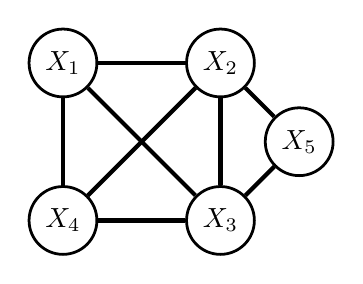
\begin{tikzpicture}[ugraph]
%\node[font=\Large] at (1.2,2.8) {Undirected Graph};
\node[cont] (x1) at (0,2) {$X_1$};
\node[cont] (x2) at (2,2) {$X_2$};
\node[cont] (x3) at (2,0) {$X_3$};
\node[cont] (x4) at (0,0) {$X_4$};
\node[cont] (x5) at (3,1) {$X_5$};
\draw(x1) -- (x2);\draw(x1) -- (x3); \draw(x1) -- (x4);
\draw(x2) -- (x3); \draw(x2) -- (x4);
\draw(x3) -- (x4); \draw(x2)--(x5);\draw(x3)--(x5);
\end{tikzpicture}}
\end{center}
\end{question}



\begin{question}
Consider the following definitions.  
A vertical bar separates alternatives. For instance, $gray  \mid grey$ defines the set \{$gray$, $grey$\}.
Parentheses are used to define the scope and precedence of the operators (among other uses). For example, $gray \mid grey$ and $gr(a\mid e)y$ are equivalent patterns which both describe the set 
 \{$gray$, $grey$\}.
The quantifier $^*$ denotes that the previous element may be repeated zero or more times. 
 For example, $ab^*c$ includes $ac$, $abc$, $abbc$, $abbbc$, and so on.
\begin{enumerate}
\item
Does the set $d (a \mid bc)^*t  $ include $dat$, $daaaaat$, $dbcabct$ ?  
\item
How would you define the set of all binary representations of natural numbers (i.e., 0, 1, 10, 11, ... ) ?
\end{enumerate}
\end{question}















\end{document}
